\documentclass{article}
\usepackage{latexsym}
\usepackage{amsmath}
\usepackage[a4paper]{geometry}
\usepackage{fullpage}
\usepackage{hyperref}
\usepackage{booktabs}
\usepackage{graphicx}
\usepackage{tikz}
\usepackage{xcolor}
\usepackage[export]{adjustbox}
\usepackage{comment}
\usepackage{subcaption}
\usepackage[style=iso]{datetime2}
%\usetikzlibrary{calc}
\usetikzlibrary{arrows,positioning} 
\tikzset{
    %Define style for course boxes
    courseboxv/.style={
           rectangle,
           draw=blue!50!black, very thick,
           fill=blue!10,
           minimum height=8cm,
           minimum width=4cm,
           text width=3.9cm,
           text centered,
           font=\bfseries\sffamily},
    courseboxh/.style={
           courseboxv,
           minimum height=4cm,
           minimum width=8cm,
           text width=7.9cm},
    courseboxhh/.style={
           courseboxh,
           minimum height=4cm,
           minimum width=16cm,
           text width=15.9cm}
}
\def\frameseparation{1.5cm}
\def\scalingfactor{.8}

\newcommand{\secref}[1]{Section~\ref{sec:#1}}
\newcommand{\secreff}[2]{Sections \ref{sec:#1} and \ref{sec:#2}}
\newcommand{\eqnref}[1]{Equation~\eqref{eq:#1}}
\newcommand{\eqnreff}[2]{Equations \eqref{eq:#1} and \eqref{eq:#2}}
\newcommand{\eqnrefff}[3]{Equations \eqref{eq:#1}, \eqref{eq:#2} and \eqref{eq:#3}}
\newcommand{\figref}[1]{Figure \ref{fig:#1}} 
\newcommand{\figreff}[2]{Figures \ref{fig:#1} and \ref{fig:#2}}
\newcommand{\figrefff}[3]{Figures \ref{fig:#1}, \ref{fig:#2} and \ref{fig:#3}}
\newcommand{\tabref}[1]{Table~\ref{tab:#1}}
\newcommand{\tabreff}[2]{Tables~\ref{tab:#1} and \ref{tab:#2}}
\newcommand{\tabrefff}[3]{Tables~\ref{tab:#1}, \ref{tab:#2} and \ref{tab:#3}}

\def\year{2024--2025}
\title{EITA65 Design of Systems for Digital Transformation\\\year}
%\title{EITA65 Digitalisering -- realisering och systemdesign med användarperspektiv\\\year}
\author{\huge The Raspberry Pi\\Raspberry Pi Project -- Part 1}
%\\Version \DTMnow}
\date{}

\begin{document}
\newgeometry{left=2.5cm,right=2.5cm,bottom=1.5cm}% for placing course schematic lower on first page
\clearpage\maketitle
\thispagestyle{empty}% to remove page numbering on first page

\begin{itemize}
\item This project will be done individually, but you will work \textit{together} in groups of 3 or 4.
\item You will not get detailed step-by-step instructions. Figuring out how to reach the goal is part of the project. (being a collaborative doer)
\item The results of this project part will be used in the next, so document your work.
\end{itemize}

\vspace{.1cm}
\begin{center}
\begin{tabular}{l}
\toprule[1.5pt]
\parbox{0.8\linewidth}{
\vspace{.2cm}{\Large Learning goals:}
\begin{itemize}
\item Becoming familiar with the Raspberry Pi 4
  \begin{itemize}
  \item Getting some hands-on experience with the Raspberry Pi.
  \item Installing and updating an operating system.
  \item Understanding the package system.
  \end{itemize}
\item Practicing collaboration skills.
\end{itemize}}\\
\bottomrule[1.5pt]
\end{tabular}
\end{center}
\vfill
\begin{center}
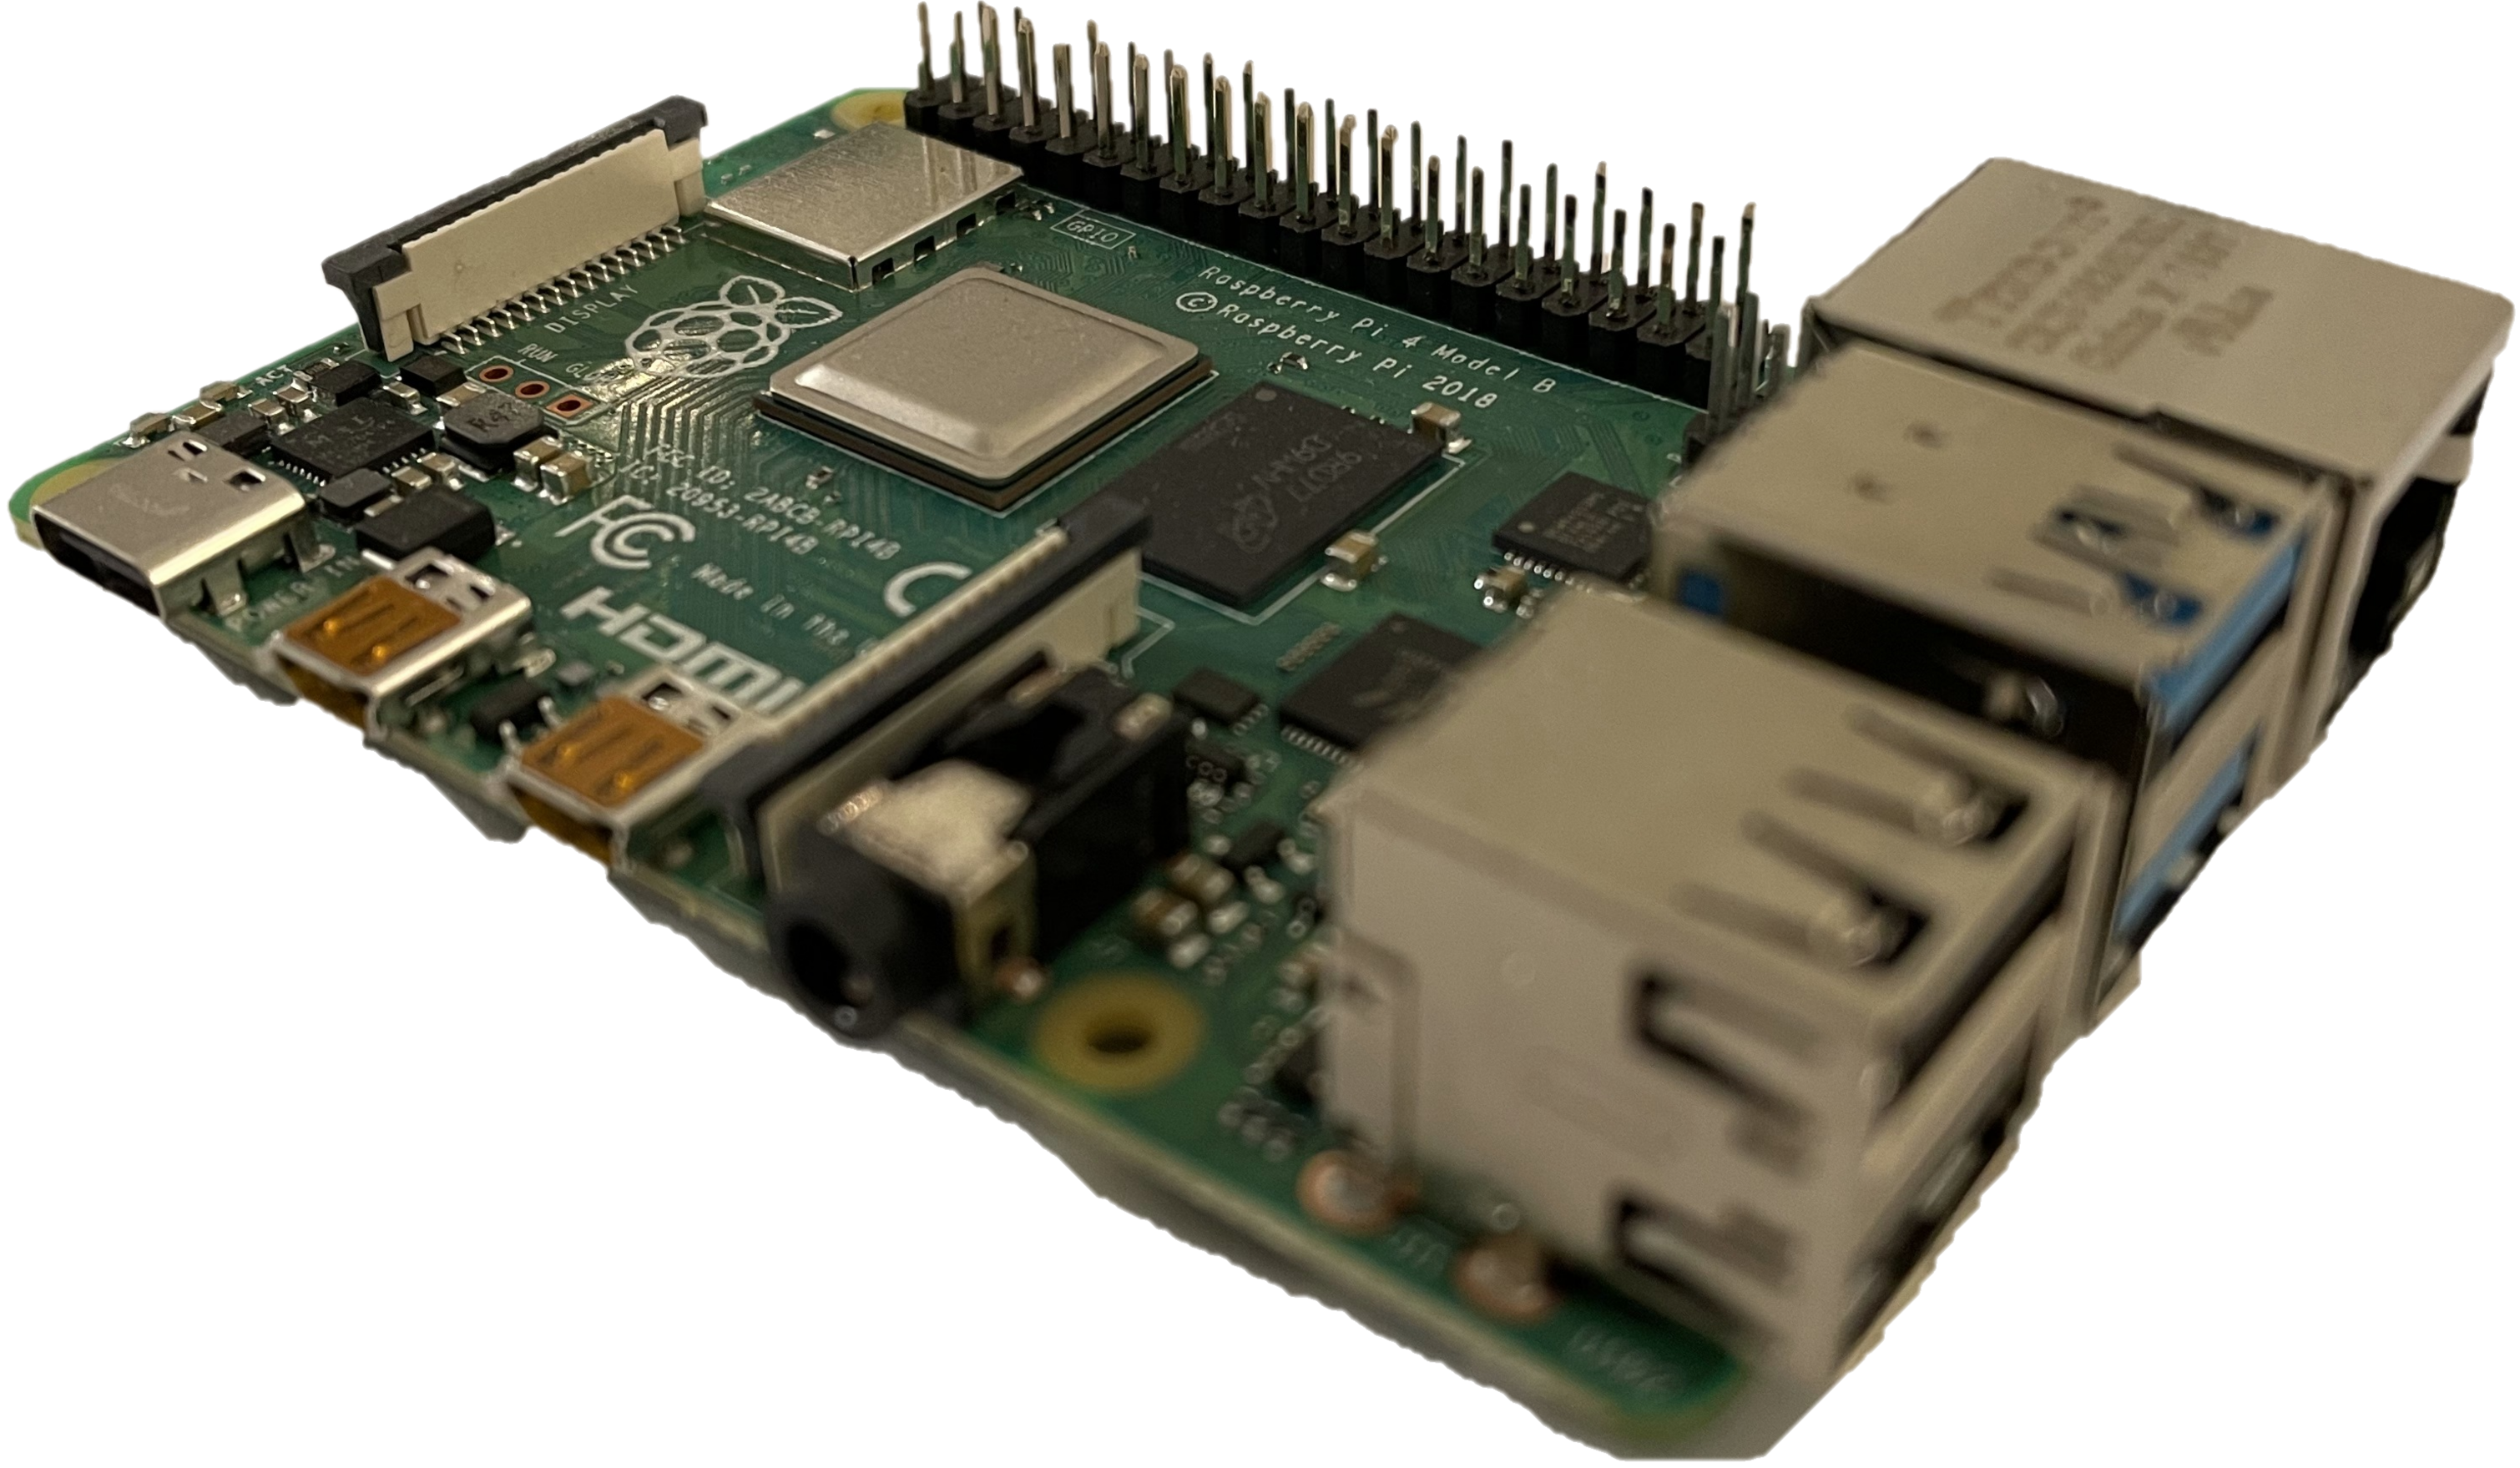
\includegraphics[width=120mm]{rpi4_no_bg.png}
\end{center}
\vspace{2cm}

\begin{comment}
\begin{center}
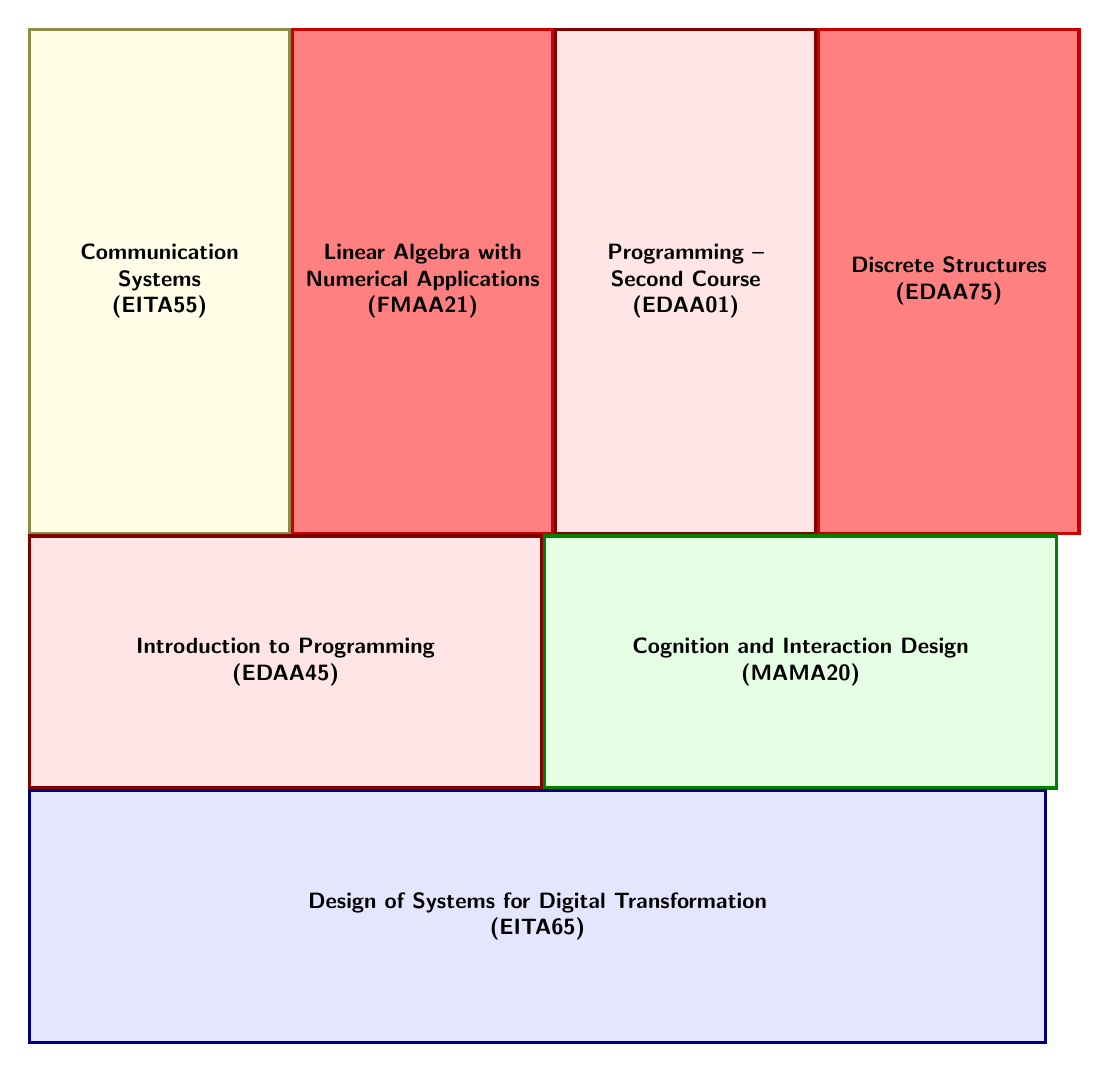
\begin{tikzpicture}[>=latex, node distance=0cm,scale=\scalingfactor,every node/.style={scale=\scalingfactor}]
\node[courseboxv, draw=yellow!50!black, fill=yellow!10] (EITA55) {Communication Systems\\(EITA55)};
\node[courseboxv, draw=red!80!black, fill=red!50, anchor=west] (FMAA21) at (EITA55.east){Linear Algebra with Numerical Applications\\(FMAA21)};
\node[courseboxv, draw=red!50!black, fill=red!10, anchor=west] (EDAA01) at (FMAA21.east){Programming -- Second Course\\(EDAA01)};
\node[courseboxv, draw=red!80!black, fill=red!50, anchor=west] (EDAA75) at (EDAA01.east){Discrete Structures\\(EDAA75)};
%\node[courseboxh, preaction={clip, postaction={fill=red!10, draw=red!50!black, line width=2mm}}, anchor=north west] (EDAA45) at (EITA55.south west){Introduction to Programming\\(EDAA45)};
\node[courseboxh, draw=red!50!black, fill=red!10, anchor=north west] (EDAA45) at (EITA55.south west){Introduction to Programming\\(EDAA45)};
%\node[courseboxh, draw=green!50!black, fill=green!10, anchor=west] (MAMA20) at (EDAA45.east){Cognition and Interaction Design\\(MAMA20)};
\node[courseboxh, draw=green!50!black, fill=green!10, right=of EDAA45] (MAMA20) {Cognition and Interaction Design\\(MAMA20)};
\node[courseboxhh, anchor=north west] (EITA65) at (EDAA45.south west){Design of Systems for Digital Transformation\\(EITA65)};
%\node[anchor=south east, inner sep=2pt, font=\bfseries\sffamily\scriptsize] at (EDA625.south east) {Helsingborg};
%\path[->,draw=black,dotted,thick] (EIT060.east) -- (EITF05.west);
%\path[->,draw=black,dotted,thick] (EIT060.south) -- (EITN50.north);
%\path[->,draw=black,dotted,thick] (EITF05.south) -- (EITN41.north);
%\draw[draw=blue!50!black, very thick] ($(EIT060.north west)+(-\frameseparation,\frameseparation)$) rectangle ($(EDA625.south east)+(\frameseparation,-\frameseparation)$);
\end{tikzpicture}
\end{center}
\end{comment}

\restoregeometry
\newpage


\section{Introduction}
In this project part you will get acquainted with a Raspberry Pi 4. 
In the first part you will
\begin{itemize}
\item[1.] Unpack your Pi
\item[2.] Install Raspberry Pi OS on your SD-card
\item[3.] Start your Pi for the first time!
\item[4.] Update, upgrade and install software on your Pi
\end{itemize}

\noindent You will need some things before getting started
\begin{itemize}
    \item A computer
    \item A SD-card reader (often built into a laptop)
    \item A TV/monitor with a HDMI-socket (or an other socket that you have an HDMI-adapter for)
    \item A USB-keyboard
    \item A USB-mouse
\end{itemize}



\section{What is a Raspberry Pi?}
A Raspberry Pi is a small computer that is built on a single circuit board. A Raspberry Pi has everything (well almost) that other computers have; a processor, memory and USB, ethernet and HDMI input/output sockets. Read more about your model (Raspberry Pi 4) on {\color{blue}\href{https://www.raspberrypi.org/products/raspberry-pi-4-model-b/}{Raspberry Pis official website}}.
\begin{center}
\includegraphics[width=100mm]{rpi4_top_view_no_bg.png}
\end{center}

\newpage

\section{The Lab Kit}
The lab kit consists of the Raspberry Pi 4 KIT and the Raspberry Pi SENSE HAT. 
\begin{center}
\includegraphics[width=30mm]{rpi_kit_box_no_bg.png}
\includegraphics[width=20mm]{rpi_sense_hat_box_no_bg.png}
\end{center}

\section{Unboxing the Raspberry Pi}
Your Raspberry Pi 4 KIT contains not only the actual Raspberry Pi, but also a case and a power supply for your Pi, a 16GB SD-card and a HDMI-cable.

\section{Setting up the OS}
The operating system (OS) is the software that binds everything in a computer together. It connects the USB-socket with software that wants to utilise it, e.g. software for a keyboard. Generally speaking an OS connects hardware with software/applications that the user interacts with \cite{OS}. The most common OS is Microsoft Windows, but the one we are going to use is called \emph{Raspberry Pi OS}. Raspberry Pi OS (PiOS from now on) is, as the name implies, specifically developed for a Raspberry Pi. PiOS is based on \emph{Debian}, and Debian in itself has a Linux-kernel. Now - to work! 

\begin{itemize}
\item[1.] You need to install the latest version of PiOS, and to do that you need a computer with an SD-card reader or an adapter with a SD-card reader. If you don't have one probably you have a friend who does.
\item[2.] Go to  {\color{blue}\href{https://www.raspberrypi.org/software/}{this website}} and download the Raspberry Pi Imager that suits your OS. Most of you are going to choose \emph{Download for Windows} since we all learned that Windows is the most common OS.
\item[3.] Install the file that was downloaded and follow the steps in {\color{blue}\href{https://www.youtube.com/watch?v=ntaXWS8Lk34}{this video}} to install the OS on your SD-card. Choose to install Raspberry Pi OS (64-bit). If you have any problems you can look at {\color{blue}\href{https://projects.raspberrypi.org/en/projects/raspberry-pi-setting-up/2}{this website}} for more detailed information.
\item[4.] The installation might take a while \ldots
\item[5.] When the installation is done, remove your SD-card from the computer. You are ready to start your Pi!
\end{itemize}
  
\section{Starting your Pi for the first time}
Your are (almost) ready to start your Pi! You need some things before:
\begin{itemize}
    \item A TV/monitor with a HDMI-socket (or an other socket that you have an HDMI-adapter for)
    \item A USB-keyboard
    \item A USB-mouse
    \item A power outlet to power your Pi
\end{itemize}
Now you are ready to go!
Follow {\color{blue}\href{https://projects.raspberrypi.org/en/projects/raspberry-pi-setting-up/3}{this guide}} until you have reached the part where you need to restart you Pi. Restart it! You should now boot into the PiOS desktop. Follow the instructions on the screen to do an initial setup of your Raspberry Pi. Make sure to read the following notes carefully.\\*\\*

{\bf Note 1: }\parbox[t]{14cm}{Be careful while choosing language in the initial setup. If you are using a Swedish keyboard we recommend you to choose Swedish in the language option so that the keyboard setup is Swedish while writing your password. Afterwards you switch the language to English, but keep the Swedish keyboard layout. Of course you can keep Swedish as your language, but it will be harder to search for instructions and help online since almost every guide and web-page about Raspberry Pi is in English. Look at the pictures below on how to change your languages settings (locale) after the initial setup. Also, do not forget to make sure your character set remains UTF-8.}
\begin{figure}[h]
    \centering
    \begin{subfigure}[t]{0.49\textwidth}
        \centering
        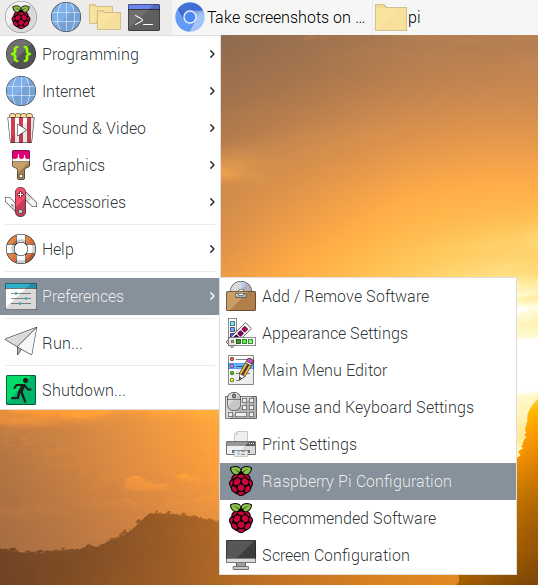
\includegraphics[width=\textwidth]{menu.png}
        \caption{Go to the menu and find \emph{Raspberry Pi Configuration}}
    \end{subfigure}
    \begin{subfigure}[t]{0.49\textwidth}
        \centering
        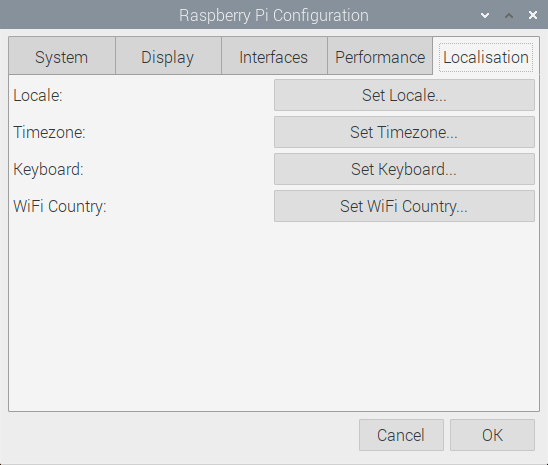
\includegraphics[width=\textwidth]{lang1.png}
        \caption{Go to the \emph{Localisation} tab and click on \emph{Set Locale}}
    \end{subfigure}
\end{figure}
\begin{figure}[h]
    \centering
    \begin{subfigure}[t]{0.49\textwidth}
        \centering
        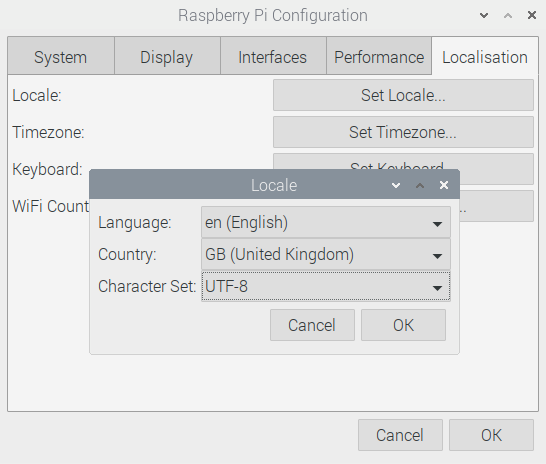
\includegraphics[width=\textwidth]{lang2.png}
        \caption{Change to your language of preference. It is good to keep the UTF-8 as your Character Set}
    \end{subfigure}
    \begin{subfigure}[t]{0.49\textwidth}
        \centering
        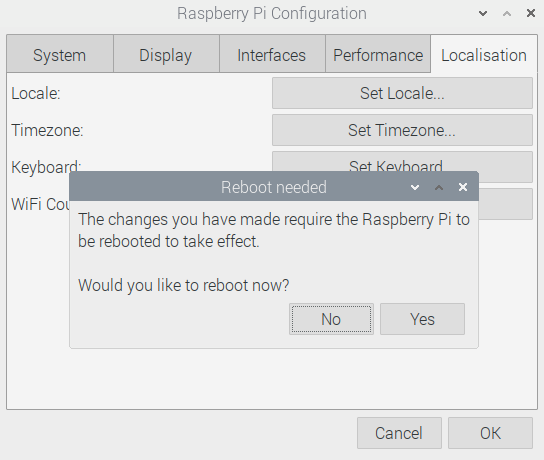
\includegraphics[width=\textwidth]{lang3.png}
        \caption{Reboot your Pi}
    \end{subfigure}
\end{figure}

\newpage

\noindent {\bf Note 2: }\parbox[t]{14cm}{You will need to connect your Pi to a network. Initially you wont be able to connect it to Eduroam or LU Guest, so please choose another network. Sharing a hotspot from your phone is a good idea. You can also try connecting using an ethernet cable directly to your router if possible. If so, skip WiFi setup for now.  Try to use internet to see if it works. If neither of these routes are available to you you can skip connecting to a network for now and then connect to Eduroam once the setup is finished. In such a case you will also need to skip software update during setup. You will find how to connect to Eduroam below.}

\vspace{2mm}

\noindent {\bf Note 3: }\parbox[t]{14cm}{If you have managed to connect to a network you will be asked if you want to enable Raspberry Pi Connect. Raspberry Pi Connect is a service which will make it possible for you to work with your Raspberry Pi via a web browser on another computer without connecting a screen/keyboard/mouse. We will not use or talk about it during the course but you might find it useful anyway. You can read more about it on the {\color{blue}\href{https://www.raspberrypi.com/documentation/services/connect.html}{Raspberry Pi documentation web site}} and decide if you want to enable it (or perhaps do it later)}.


\section{Connecting to Eduroam}

If you are working at home and have managed to connect to a network you can skip this section and return to it when you want to connect you Raspberry Pi to Eduroam.

\begin{enumerate}
    \item[1.] Click on the network icon in the upper right corner of the screen. It will either look as a blue WiFi symbol or a symbol with two red crosses depending on your connection status. 
    \item[2.] Choose eduroam in the menu that appears.
    \item[3.] Fill out the form that appears according to figure \ref{fig:eduroam}.
    \item[4.] Click Connect.
\end{enumerate}

\begin{figure}[h]
    \centering
    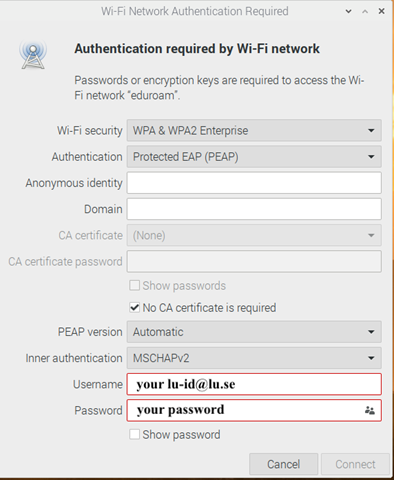
\includegraphics[width=90mm]{eduroam.png}
    \caption{How to enter your credentials into the new network manager}
    \label{fig:eduroam}
\end{figure}



\section{Understanding the packaging system}
The operating system (OS) you are using does not update itself, like if you are using Windows, the computer sometimes download and installs updates on its own. The Raspberry Pi OS gives you more control over your computer as to how, what and when you want to expand and upgrade your OS.

Software functionality is bundled in packages, and you can install the ones that are useful to you. A package handler makes it easy to update, install and remove packages. There are several such package handlers, such as \verb!apt!, \verb!apt-get! and \verb!apt-cache!, but they are all very similar in usage.

Normally, you always update your OS before you install a new software/packages.\\
%\newline
Try it out! Open a terminal by clicking on the Terminal icon in the upper left corner. It should look like in \figref{terminal}.
\begin{figure}[h]
    \centering
    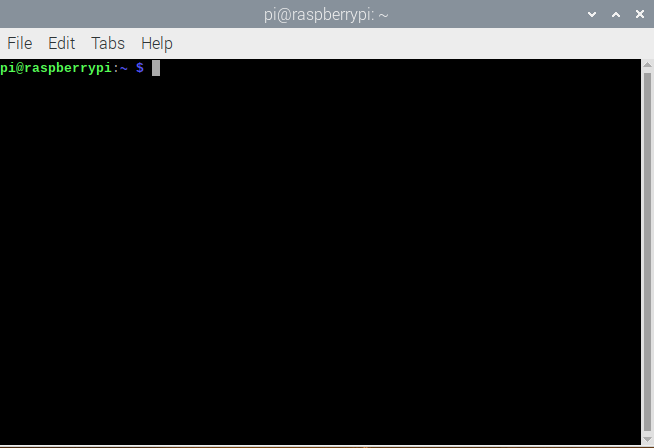
\includegraphics[width=100mm]{terminal.png}
    \caption{A terminal window}
    \label{fig:terminal}
\end{figure}
\newline
You update the OS by writing command \eqref{eq:update} and pressing enter. The command tells the OS to download all the available updates to your computer. Please make sure that you are connected to the internet. You might get the question \texttt{Do you want to continue [Y/n]} if there is something to download. Type y or Y (short for yes) and press enter to continue, or n or N (short for no) to cancel.
\begin{equation}
\label{eq:update}
\verb!sudo apt update!
\end{equation}
After the first command you always follow up by typing command \eqref{eq:upgrade}. This command tells the OS to actually install all the downloaded updates. Here you can also get the question if you want to continue, answer y in that case. 
\begin{equation}
\label{eq:upgrade}
\verb!sudo apt full-upgrade!
\end{equation}
Command \eqref{eq:clean} you can use if you have limited space and need to free up some more. Try it out!
\begin{equation}
\label{eq:clean}
\verb!sudo apt clean!
\end{equation}
Sometimes you need to reboot your Pi in order for the changes to kick in. Try command \eqref{eq:reboot} or use the menu option (click on the raspberry in the top left corner of your screen) \emph{shutdown} to reboot.
\begin{equation}
\label{eq:reboot}
\verb!sudo reboot!
\end{equation}
%\newline
\verb!sudo! is short for \verb!super user do! and gives the current user root privileges. If you are using Windows maybe sometimes you get a pop-up windows saying that you need administrator privileges to continue, and you could say that root privileges is something similar in our OS. You often have to use \verb!sudo! when you are making permanent changes to your OS \cite{sudo}. The webcomic XKCD made a short comic \cite{xkcd} about the command that you can see in \figref{xkcd}.
\begin{figure}[ht]
    \centering
    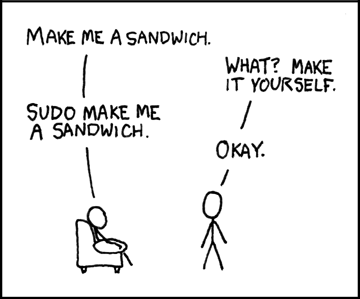
\includegraphics[width=100mm]{sandwich.png}
    \caption{XKCDs comic\#149}
    \label{fig:xkcd}
\end{figure}

\section{Task: write a shell script}
\noindent Shell scripts are good for automating tasks by running several commands consecutively, in a sequence. Your next task is now to write a shell script that runs all of commands \eqref{eq:update} to \eqref{eq:reboot} consecutively in a sequence for a full OS update cycle. You will need to find out exactly how to do this on your own, but a good indication that you are on the right track is that the instructions you find explains what a \textit{shebang} is, and probably also mention the \verb!chmod! command. Name your shell script file \verb!update_os.sh!, and make sure that it works by executing (running) it.

Using your new shell script knowledge, you can now both automate tasks and avoid retyping complicated commands.

% \section{Install a new network manager}


% When you boot into the Raspberry Pi your the first time, you may not able to connect to the university WiFi \emph{Eduroam}. This is due to the simple network managing service used by PiOS that cannot set up a complex enterprise wireless network like Eduroam. The simplest way to solve this is to install another network manager with the following steps:
% \begin{itemize}

%     \item[1.] Make sure you can access internet when you boot into your Raspberry Pi. Use your own WiFi at home or maybe start a hotspot from your phone.
%     \item[2.] Open a terminal
%     \item[3.] Use command \eqref{eq:update} and \eqref{eq:upgrade} that you just learned.
%     \item[4.] Install the new network manager using command \eqref{eq:install}
% \end{itemize}
% \begin{equation}
% \label{eq:install}
% \verb!sudo apt-get install network-manager network-manager-gnome!
% \end{equation}
% \begin{itemize}
%     \item[5.] Stop the old manager and start the new one by using command \eqref{eq:disable} and \eqref{eq:enable}
% \end{itemize}
% \begin{equation}
% \label{eq:disable}
% \verb!sudo systemctl disable --now dhcpcd!
% \end{equation}
% \begin{equation}
% \label{eq:enable}
% §\verb!sudo systemctl enable --now NetworkManager!
% \end{equation}
% \begin{itemize}
%     \item[6.] Reboot the system. You should see another network manager icon in your menu bar and you can connect to Eduroam via it. Figure \ref{fig:eduroam} shows how to enter your username and password.
% \end{itemize}
% \begin{figure}[h]
%     \centering
%     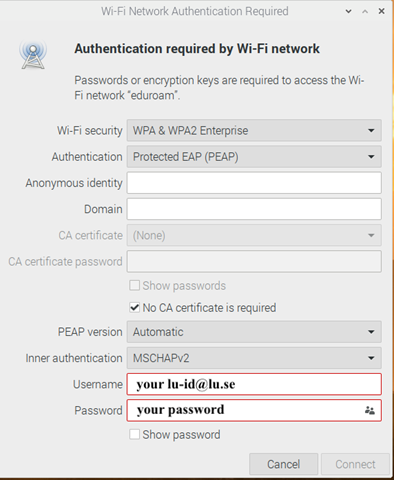
\includegraphics[width=100mm]{eduroam.png}
%     \caption{How to enter your credentials into the new network manager}
%     \label{fig:eduroam}
% \end{figure}

% {\bf Note: }\parbox[t]{14cm}{The time synchronization service on PiOS might also be poor. You may get problems to access internet if your system time is not correct. In case of problems you can set up your system time manually via command \eqref{eq:false}, \eqref{eq:settime} and \eqref{eq:true}}
% \begin{equation}
% \label{eq:false}
% \verb!sudo timedatectl set-ntp false!
% \end{equation}
% \begin{equation}
% \label{eq:settime}
% \verb!sudo timedatectl set-time "Y-M-D HH:mm"!
% \end{equation}
% \begin{equation}
% \label{eq:true}
% \verb!sudo timedatectl set-ntp true!
% \end{equation}

\section{Lab Goal}
{\textcolor{red}{You will need to show the TAs that your Pi was properly installed, updated and can connect to Eduroam.}}

\section{Helpful Hints}

{\bf Hint 1: }\parbox[t]{14cm}{To avoid rewriting many commands in the terminal, you can use the keys \texttt{arrow up} and \texttt{arrow down} to go back and forth between the commands that you just wrote.}\\
{\bf Hint 2: }\parbox[t]{14cm}{To paste commands into the terminal you can use \texttt{Ctrl + Shift + V}}\\
{\bf Hint 3: }\parbox[t]{14cm}{Use \textit{Tab} to auto-complete the command in the terminal}\\
{\bf Hint 4: }\parbox[t]{14cm}{To avoid rewriting many commands, it can be a good idea to write all steps in a batch-file or shell script. Then you can also reuse the batch file for the second project.}
\vspace{1cm}
\begin{center}
\huge Good luck!
\end{center}

\newpage

\begin{thebibliography}{10}
\bibliographystyle{plain}
\bibitem{iso-date-time} ISO 8601 -- Date and Time Format, \url{https://www.iso.org/iso-8601-date-and-time-format.html}, last accessed on 2021-09-21.
\bibitem{OS} Operating system, wikipedia, \url{https://en.wikipedia.org/wiki/Operating_system}, last accessed on 2021-09-15.
\bibitem{sudo} Using Linux -- The sudo command, \url{https://www.raspberrypi.org/documentation/computers/using_linux.html}, last accessed on 2021-09-15.
\bibitem{xkcd} XKCD -- Sandwich, \url{https://xkcd.com/149/}, last accessed on 2021-09-15.
\end{thebibliography}

\end{document}
